\documentclass[UTF8,11pt]{ctexart}
\usepackage[a4paper,margin=22mm]{geometry}
\usepackage{graphicx,enumitem,amssymb,tabularx}
\usepackage[normalem]{ulem}
\usepackage{xeCJKfntef}
\setlength{\parindent}{0pt}
\setlength{\parskip}{.6em}
\sloppy
\begin{document}
\section*{2019年12月英语六级真题(第3套)}
\subsection*{2019年12月英语六级考试试题第3套}


\subsection*{\textbf{Part II} \textbf{Listening Comprehension} \textbf{(30 minutes)}}


\noindent
\includegraphics[width=\linewidth,height=.8\textheight,keepaspectratio]{2019-12-03.assets/char-001-line-002.png}\par

\subsection*{\textbf{Part III} \textbf{Reading Comprehension} \textbf{( 40 minutes)}}


\subsection*{\textbf{Section A}}


\textbf{Directions : }\textit{In this section , there is a passage with ten blanks. You are required to select one word for}


\textit{each blank from a list of choices given in a word bank following the passage. Read the}


\subsection*{\textit{passage through carefully before making your choices. Each choice in the bank is identified}}


\textit{by a letter. Please mark the corresponding letter for each item on }\textbf{\textit{Answer Sheet 2 }}\textit{with a}


\textit{single line through the centre. You may not use any of the words in the bank more than} \textit{once.}


The number of devices you can talk to is multiplying-first it was your phone, then your car, and now you can tell your kitchen appliances what to do. But even without gadgets that understand our spoken commands, research suggests that, as bizarre as it sounds, under certain 26 , people regularly ascribe human traits to everyday objects.


Sometimes we see things as human because we are 27 . In one experiment, people who reported feeling isolated were more likely than others to attribute 28 to various gadgets. In tum, feeling close to objects can 29 loneliness. When college students were reminded of a time they had been 30 in a social setting, they compensated by exaggerating their number of friends-unless they were first given tasks that caused them to interact with their phone as if it had human qualities. According to the researchers, the participants' phones 3 1 substituted for real friends.


At other times, we personify products in an effort to understand them. One study found that three in four respondents yelled at their computer. Further, the more their computer gave them problems, the more likely the respondents were to report that it had its own " beliefs and 32


So how do people assign traits to an object? In part, we rely on looks. On humans, wide faces are 33 with dominance. Similarly, people rated cars, clocks, and watches with wide faces as more dominant-looking than narrow-faced ones, and preferred them-especially in 34 situations. An analysis of car sales in Germany found that cars with \textit{grilles }( ctt ,\#JJt) that were upturned like smiles sold best. The purchasers saw this 35 as increasing a car's friendliness.


第 1／9页


\begin{itemize}[leftmargin=2em,itemsep=.2em,topsep=.4em]\item[A.] alleviate
\item[B.] apparently
\item[C.] arrogant
\item[D.] associated
\item[E.] circumstances
\item[F.] competitive
\item[G.] conceded
\item[H.] consciousness
\item[I.] desires
\item[J.] excluded
\item[K.] feature
\item[L.] lonely
\item[M.] separate
\item[N.] spectacularly
\item[O.] warrant
\end{itemize}

\subsection*{\textbf{Section B}}


\textbf{Directions : }\textit{In this section , you are going to read a passage with ten statements attached to it. Each}


\textit{statement contains information given in one of the paragraphs. Identify the paragraph from}


\textit{which the information is derived. You may choose a paragraph more than once. Each}


\textit{paragraph is marked with a letter. Answer the questions by marking the corresponding letter}


\textit{on }\textbf{\textit{Answer Sheet 2.}}


\textbf{Why More Farmers Are Making The Switch to Grass-Fed Meat and Dairy}


[ A] Though he didn't come from a farming family, from a young age Tim Joseph was fascinated by


the idea of living off the land. Reading magazines like \textit{The Stockman Grass Farmer }and \textit{Graze, }he got hooked on the idea of grass-fed agriculture. The idea that all energy and wealth comes from the sun really intrigued him. He thought the shorter the distance between the sun and the end product, the higher the profit to the farmer.


\noindent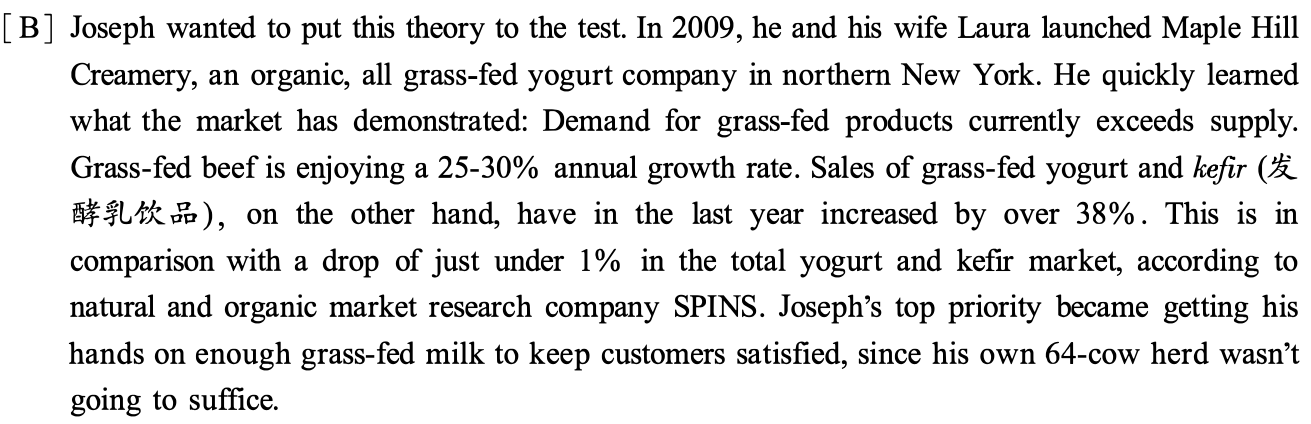
\includegraphics[width=\linewidth,height=.8\textheight,keepaspectratio]{2019-12-03.assets/char-002-line-010.png}\par

[ C] His first partnership was with Paul and Phyllis Amburgh, owners of the Dharma Lea farm in


New York. The Amburghs, too, were true believers in grass-fed. In addition to supplying milk from their own 85-head herd, they began to help other farmers in the area convert from conventional to certified organic and grass-fed in order to enter the Maple Hill supply chain.


第 2／9页


Since 20 10, the couple has helped 125 small dairy farms convert to grass-fed, with more than 80\% of those farms corning on board during the last two years.


[ D] All this conversion has helped Maple Hill grow 40-50\% every year since it began, with no end


in sight. Joseph has learned that a farmer has to have a certain mindset to successfully convert. But convincing open-minded dairy people is actually not that hard, when you look at the economics. Grass-fed milk can fetch up 2.5 times the price of conventional milk. Another factor is the squeeze that conventional dairy farmers have felt as the price of grain they feed their cows has gone up, tightening their profit margins. By replacing expensive grain feed with regenerative management practices, grass-fed farmers are insulated from jumps in the price of feed. These practices include grazing animals on grasses grown from the pastureland's natural seed bank, and fertilized by the cows' own fertilizer.


[ E] Champions of this type of regenerative grazing also point to its animal welfare, climate and


health benefits: Grass-fed animals live longer out of confinement. Grazing herds stimulate \textit{microbial }(,\{;ft ± 4h al.] ) activity in the soil, helping to capture water and separate carbon. And grass-fed dairy and meat have been shown to be higher in certain nutrients and healthy fats.


[ F ] In the grass fed system, farmers are also not subject to the wildly fluctuating milk prices of the


international commodity market. The unpredictability of global demand and the lag-time it takes to add more cows to a herd to meet demand can result in events like the recent cheese surplus. Going grass-fed is a safe refuge, a way for family-scale farms to stay viable. Usually a farmer will get to the point where financially, what they're doing is not working. That's when they call Maple Hill. If the farm is well managed and has enough land, and the desire to convert is sincere, a relationship can begin. Through regular regional educational meetings, a large annual meeting, individual farm visits and thousands of phone calls, the Amburghs pass on the principles of pasture management. Maple Hill signs a contract pledging to buy the farmer's milk at a guaranteed base price, plus quality premiums and incentives for higher protein, butter-fat and other solids.


[ G] While Maple Hill's conversion program is unusually hands-on and comprehensive, it's just one


of a growing number of businesses committed to slowly changing the way America farms. Joseph calls sharing his knowledge network through peer-to-peer learning a core piece of the company's culture. Last summer, Massachusetts grass-fed beef advocate John Smith launched Big Picture Beef, a network of small grass-fed beef farms in New England and New York that is projected to bring to market 2,500 head of cattle from 125 producers this year. Early indications are that Smith will have no shortage of farm members. Since he began to informally announce the network at farming conferences and on social media, he's received a steady stream of inquiries from interested farmers.


第 3／9页


\noindent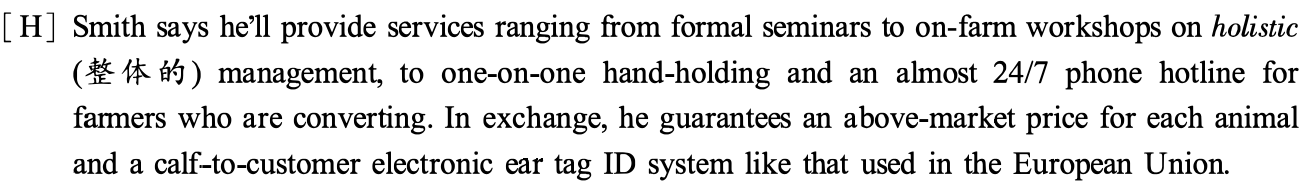
\includegraphics[width=\linewidth,height=.8\textheight,keepaspectratio]{2019-12-03.assets/char-004-line-000.png}\par

[ I] Though advocates portray grass fed products as a win-win situation for all, they do have


downsides. Price, for one, is an issue. Joseph says his products are priced 10-20\% above organic versions, but depending on the product chosen, compared to non-organic conventional yogurt, consumers could pay a premium of 30-50\% or more for grass-fed. As for the meat, Smith says his grass-fed hamburger will be priced 20-25\% over the conventional alternative. But a look at the prices on online grocer Fresh Direct suggests a grass-fed premium of anywhere from 35-60\% .


[ J] And not every farmer has the option of going grass-fed. For both beef and dairy production it


requires, at least in the beginning, more pastureland. Grass-fed beef production tends to be more labor-intensive as well. But Smith counters that if you factor in the hidden cost of government corn subsidies, environment degradation, and decreased human heath and animal welfare, grass- fed is the more cost-effective model. " The sun provides the lowest cost of production and the cheapest meat," he says.


\noindent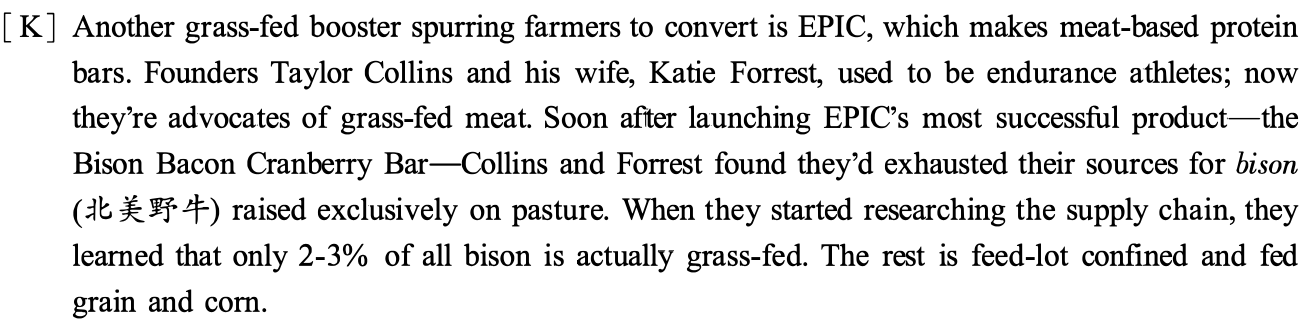
\includegraphics[width=\linewidth,height=.8\textheight,keepaspectratio]{2019-12-03.assets/char-004-line-005.png}\par

[ L] But after General Mills bought EPIC in 2016, Collins and Forrest suddenly had the resources


they needed to expand their supply chain. So the company teamed up with Wisconsin-based rancher Northstar Bison. EPIC fronted the money for the purchase of \$ 2.5 million worth of young bison that will be raised according to its grass-fed protocols, with a guaranteed purchase price. The message to young people who might not otherwise be able to afford to break into the business is," ' You can purchase this \$ 3 million piece of land here, because I'm guaranteeing you today you'll have 1 ,000 bison on it.' We're bringing new blood into the old, conventional farming ecosystem, which is really cool to see," Collins explains.


36. Farmers going grass-fed are not affected by the ever-changing milk prices of the global market.


37. Over the years, Tim Joseph's partners have helped many dairy farmers to switch to grass-fed.


第 4／9页


38. One advocate believes that many other benefits should be taken into consideration when we assess


the cost-effectiveness of grass-fed farming.


39. Many dairy farmers were persuaded to switch to grass-fed when they saw its advantage in terms


of profits.


40. Tim Joseph's grass-fed program is only one example of how American farming practice is


changing.


41 . Tim Joseph was fascinated by the notion that sunlight brings energy and wealth to mankind.


42. One problem with grass-fed products is that they are usually more expensive than conventional


ones.


43. Grass fed products have proved to be healthier and more nutritious.


44. When Tim Joseph started his business, he found grass-fed products fell short of demand.


45. A snack bar producer discovered that the supply of purely grass-fed bison meat was scarce.


\subsection*{\textbf{Section C}}


\textbf{Directions }: \textit{There are 2 passages in this section. Each passage is followed by some questions or} \textit{unfinished statements. For each of them there are four choices marked A }) , \textit{B }) , \textit{C ) and}


\begin{itemize}[leftmargin=2em,itemsep=.2em,topsep=.4em]\item[D.] . \textit{You should decide on the best choice and mark the corresponding letter on }\textbf{\textit{Answer}} \textbf{\textit{Sheet 2 }}\textit{with a single line through the centre.}
\end{itemize}

\subsection*{\textbf{Passage One}}


\textbf{Questions 46 to 50 are based on the following passage.}


\noindent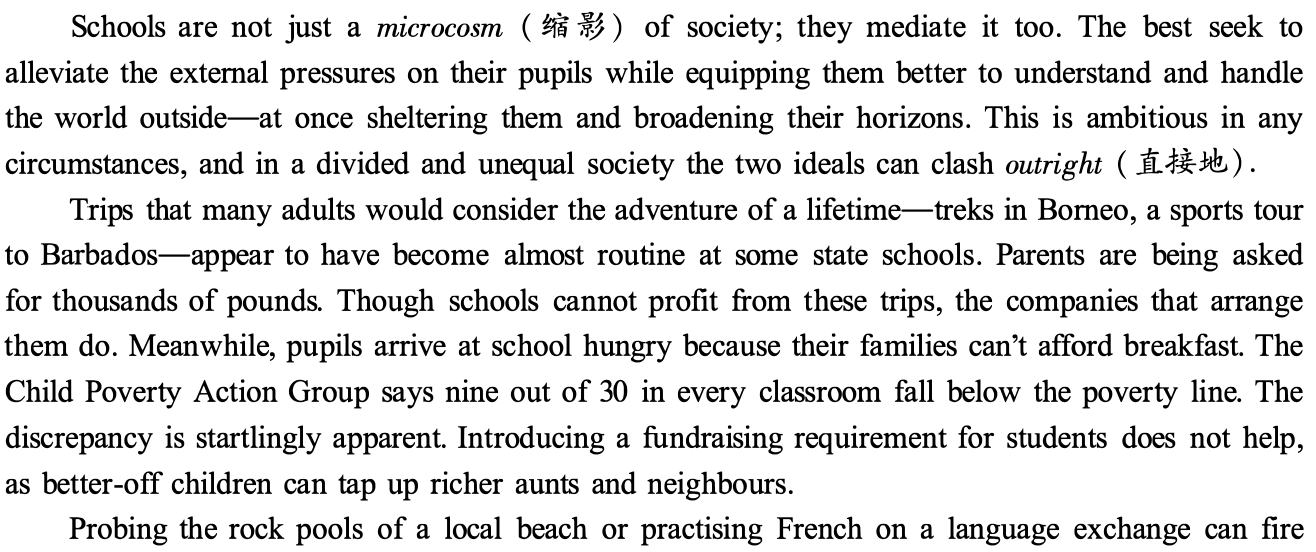
\includegraphics[width=\linewidth,height=.8\textheight,keepaspectratio]{2019-12-03.assets/char-005-line-017.png}\par

第 5／9页


\noindent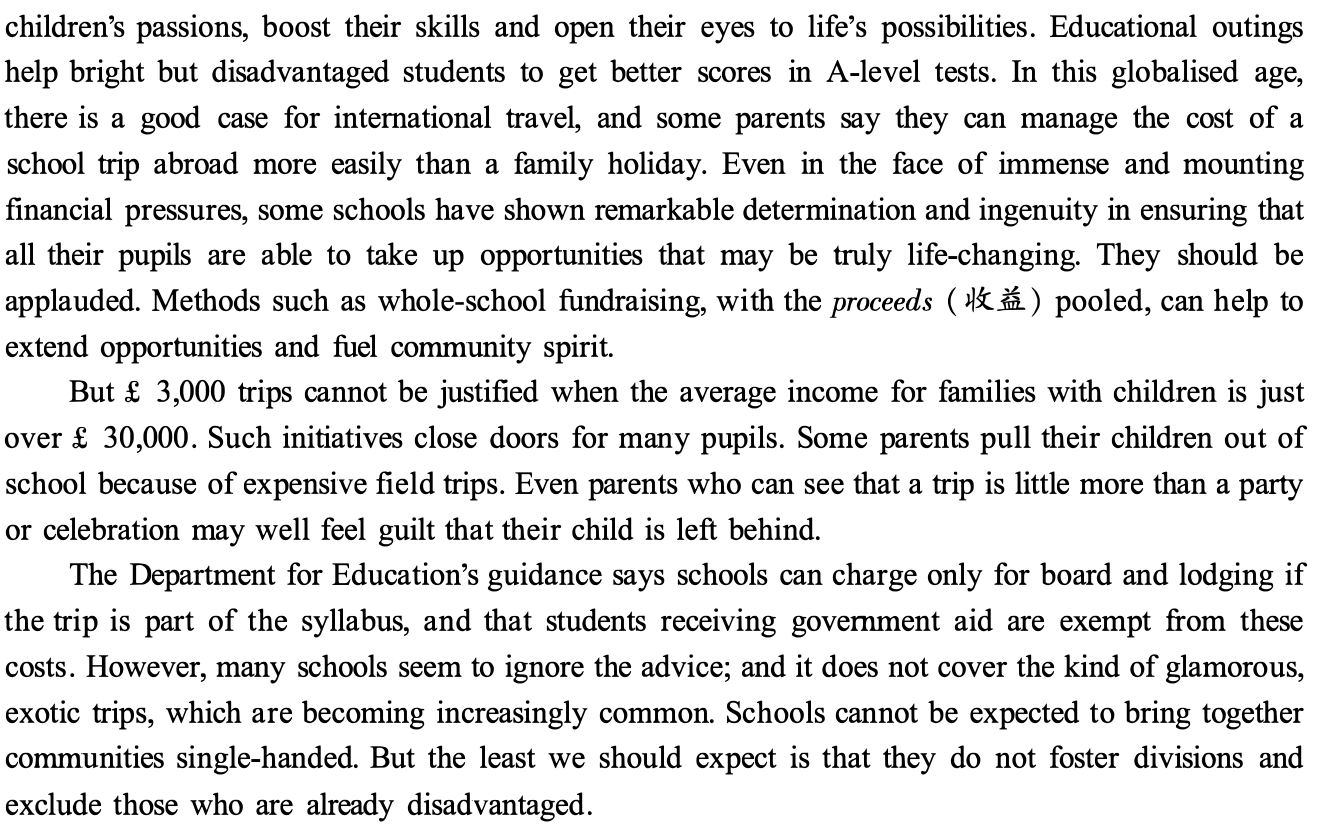
\includegraphics[width=\linewidth,height=.8\textheight,keepaspectratio]{2019-12-03.assets/char-006-line-000.png}\par

46. What does the author say best schools should do?


\begin{itemize}[leftmargin=2em,itemsep=.2em,topsep=.4em]\item[A.] Prepare students to both challenge and change the divided unequal society.
\item[B.] Protect students from social pressures and enable them to face the world.
\item[C.] Motivate students to develop their physical as well as intellectual abilities.
\item[D.] Encourage students to be ambitious and help them to achieve their goals.
\end{itemize}

47. What does the author think about school field trips?


\begin{itemize}[leftmargin=2em,itemsep=.2em,topsep=.4em]\item[A.] They enable students from different backgrounds to mix with each other.
\item[B.] They widen the gap between privileged and disadvantaged students.
\item[C.] They give the disadvantaged students a chance to see the world.
\item[D.] They only benefit students with rich relatives and neighbours.
\end{itemize}

48. What does the author suggest can help build community spirit?


\begin{itemize}[leftmargin=2em,itemsep=.2em,topsep=.4em]\item[A.] Events aiming to improve community services.
\item[B.] Activities that help to fuel students' ingenuity.
\item[C.] Events that require mutual understanding.
\item[D.] Activities involving all students on campus.
\end{itemize}

49. What do we learn about low-income parents regarding school field trips?


\begin{itemize}[leftmargin=2em,itemsep=.2em,topsep=.4em]\item[A.] They want their children to participate even though they don't see much benefit.
\item[B.] They don't want their kids to participate but find it hard to keep them from going.
\item[C.] They don't want their kids to miss any chance to broaden their horizons despite the cost.
\end{itemize}

第 6／9页


\begin{itemize}[leftmargin=2em,itemsep=.2em,topsep=.4em]\item[D.] They want their children to experience adventures but they don't want them to run risks.
\end{itemize}

50. What is the author's expectation of schools?


\begin{itemize}[leftmargin=2em,itemsep=.2em,topsep=.4em]\item[A.] Bringing a community together with ingenuity.
\item[B.] Resolving the existing discrepancies in society.
\item[C.] Avoiding creating new gaps among students.
\item[D.] Giving poor students preferential treatment.
\end{itemize}

\subsection*{\textbf{Passage Two}}


\textbf{Questions 51 to 55 are based on the following passage.}


\noindent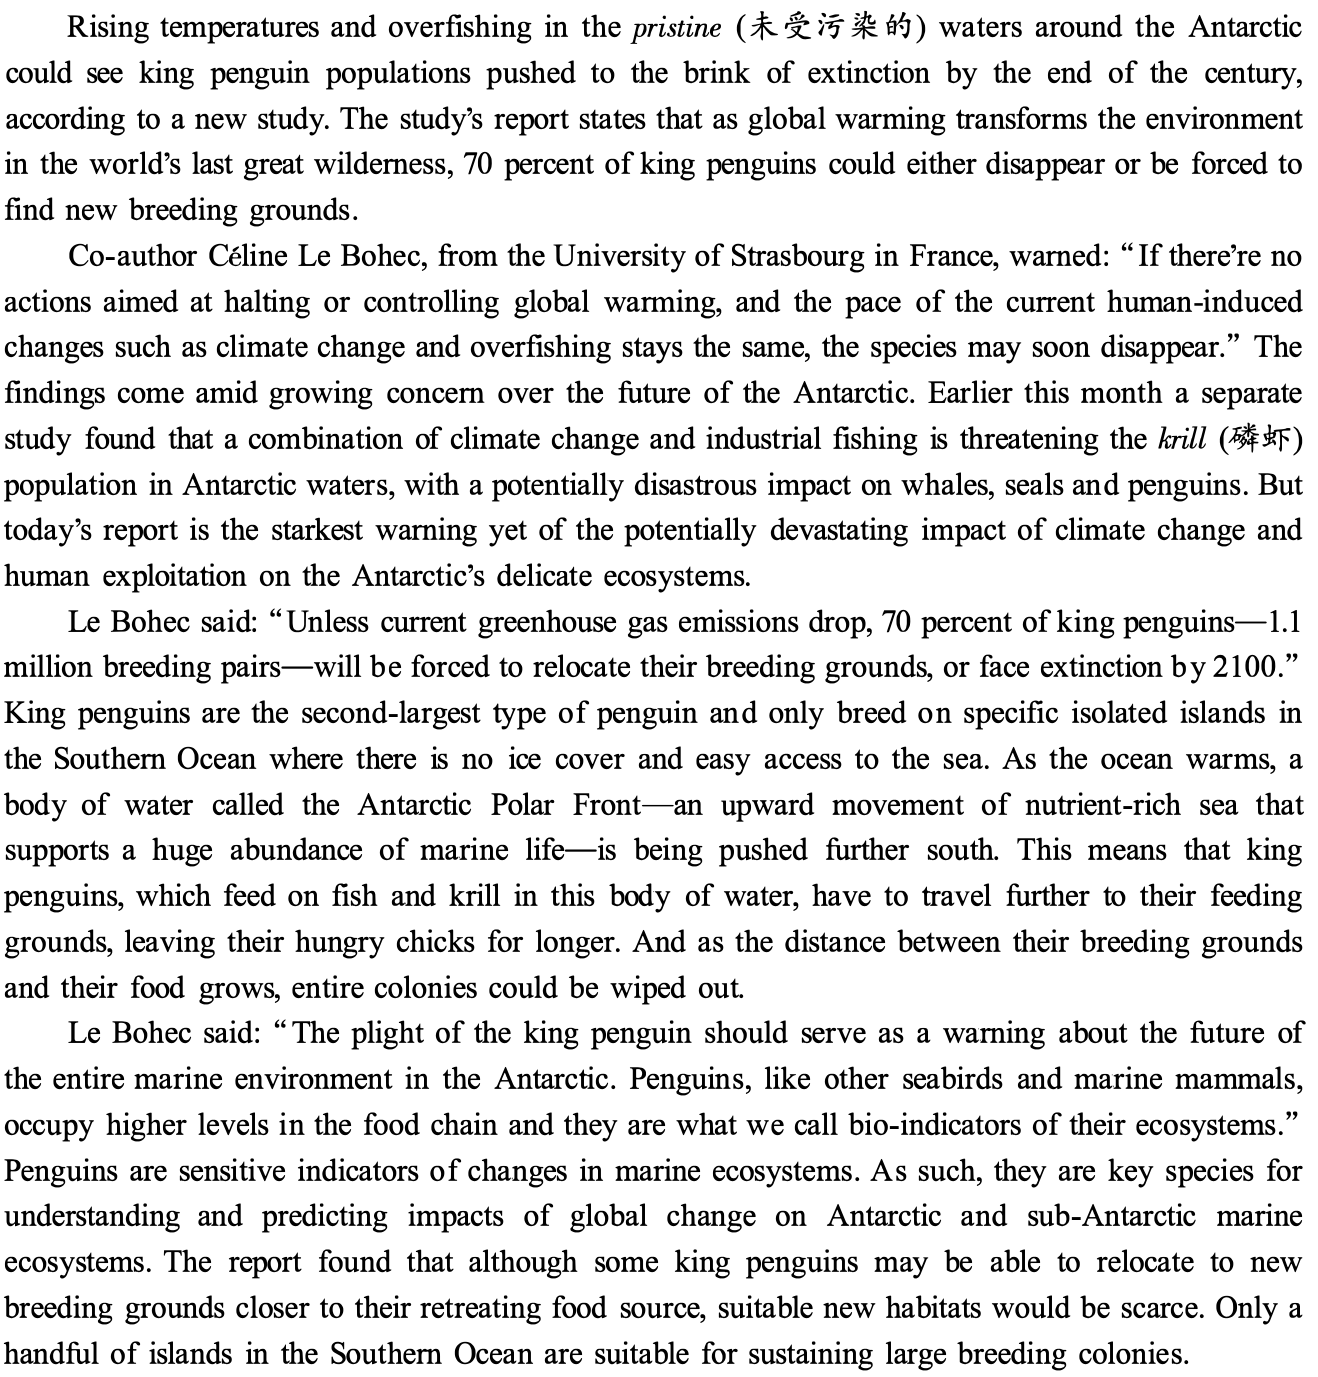
\includegraphics[width=\linewidth,height=.8\textheight,keepaspectratio]{2019-12-03.assets/char-007-line-005.png}\par

第 7／9页


\noindent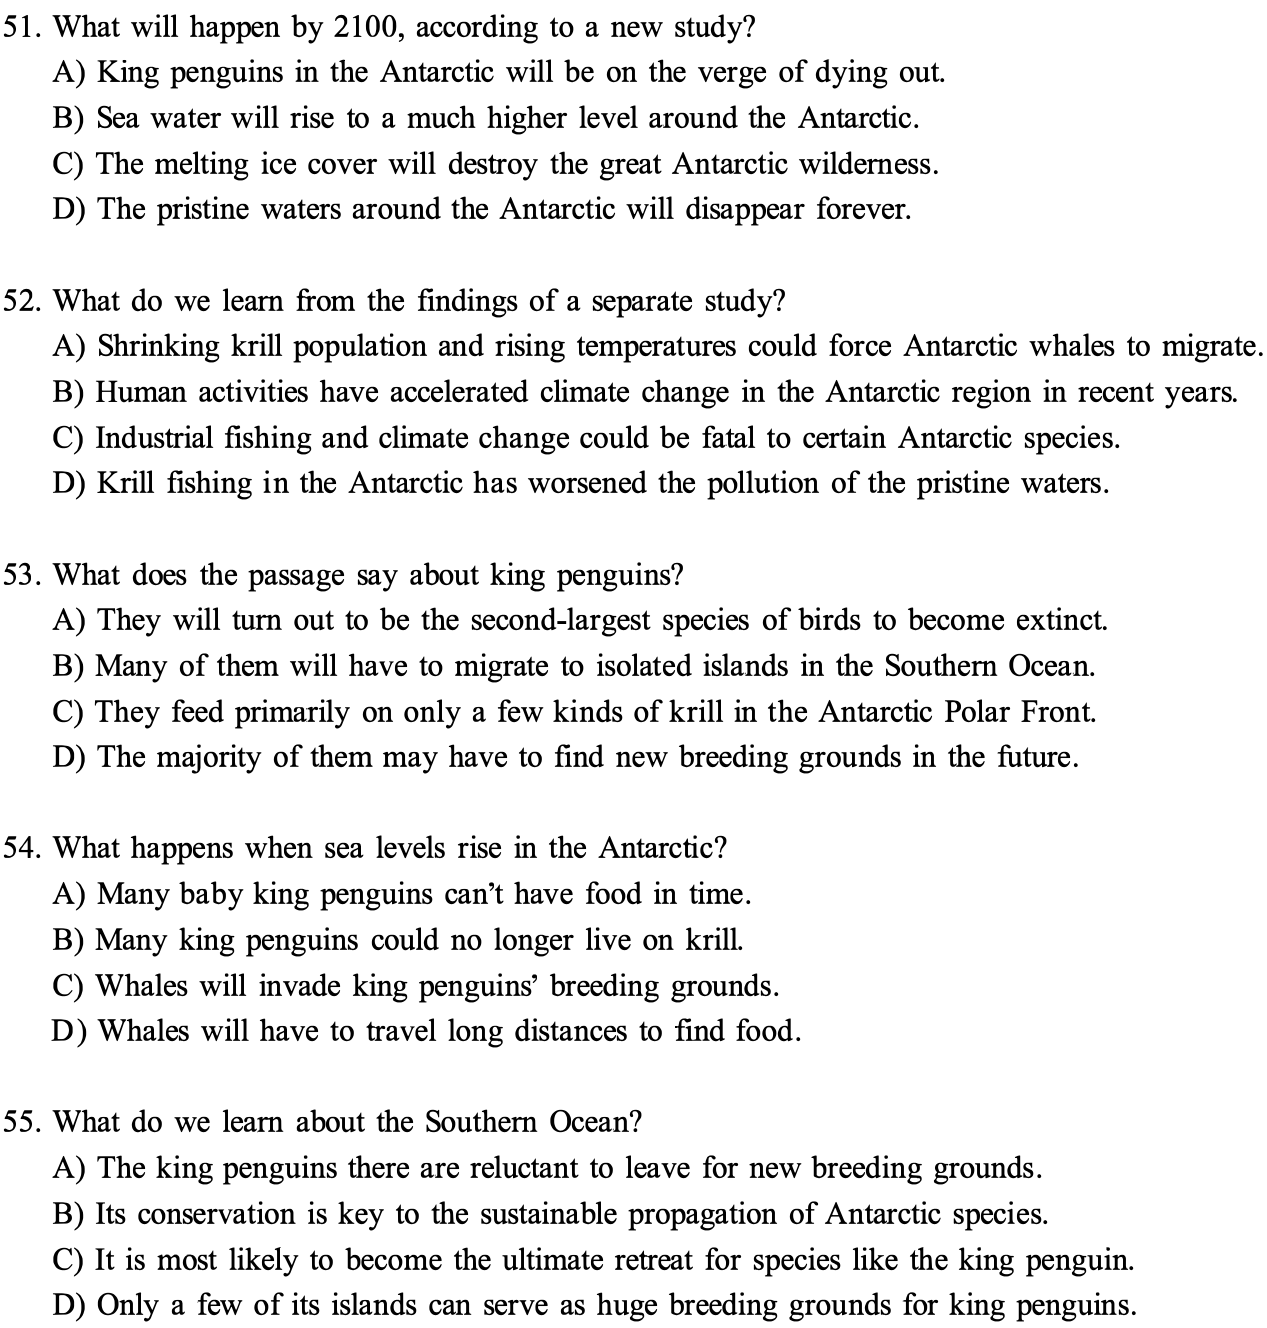
\includegraphics[width=\linewidth,height=.8\textheight,keepaspectratio]{2019-12-03.assets/char-008-line-000.png}\par

51. What will happen by 2100, according to a new study?


\begin{itemize}[leftmargin=2em,itemsep=.2em,topsep=.4em]\item[A.] King penguins in the Antarctic will be on the verge of dying out.
\item[B.] Sea water will rise to a much higher level around the Antarctic.
\item[C.] The melting ice cover will destroy the great Antarctic wilderness.
\item[D.] The pristine waters around the Antarctic will disappear forever.
\end{itemize}

52. What do we learn from the findings of a separate study?


\begin{itemize}[leftmargin=2em,itemsep=.2em,topsep=.4em]\item[A.] Shrinking krill population and rising temperatures could force Antarctic whales to migrate.
\item[B.] Human activities have accelerated climate change in the Antarctic region in recent years.
\item[C.] Industrial fishing and climate change could be fatal to certain Antarctic species.
\item[D.] Krill fishing in the Antarctic has worsened the pollution of the pristine waters.
\end{itemize}

53. What does the passage say about king penguins?


\begin{itemize}[leftmargin=2em,itemsep=.2em,topsep=.4em]\item[A.] They will turn out to be the second-largest species of birds to become extinct.
\item[B.] Many of them will have to migrate to isolated islands in the Southern Ocean.
\item[C.] They feed primarily on only a few kinds of krill in the Antarctic Polar Front.
\item[D.] The majority of them may have to find new breeding grounds in the future.
\end{itemize}

54. What happens when sea levels rise in the Antarctic?


\begin{itemize}[leftmargin=2em,itemsep=.2em,topsep=.4em]\item[A.] Many baby king penguins can't have food in time.
\item[B.] Many king penguins could no longer live on krill.
\item[C.] Whales will invade king penguins' breeding grounds.
\item[D.] Whales will have to travel long distances to find food.
\end{itemize}

55. What do we learn about the Southern Ocean?


\begin{itemize}[leftmargin=2em,itemsep=.2em,topsep=.4em]\item[A.] The king penguins there are reluctant to leave for new breeding grounds.
\item[B.] Its conservation is key to the sustainable propagation of Antarctic species.
\item[C.] It is most likely to become the ultimate retreat for species like the king penguin.
\item[D.] Only a few of its islands can serve as huge breeding grounds for king penguins.
\end{itemize}

\subsection*{\textbf{Part IV} \textbf{Translation} \textbf{(30 minutes)}}


\textbf{Directions : }\textit{For this part , you are allowed 30 minutes to translate a passage from Chinese into}


\textit{English. You should write your answer on }\textbf{\textit{Answer Sheet 2.}}


\noindent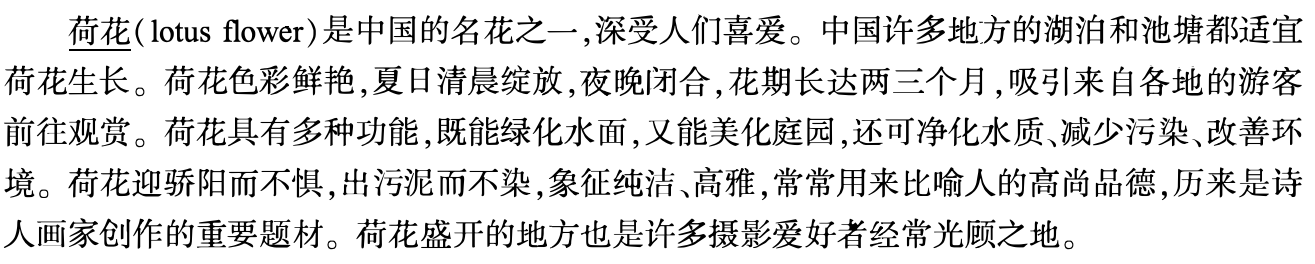
\includegraphics[width=\linewidth,height=.8\textheight,keepaspectratio]{2019-12-03.assets/char-008-line-014.png}\par

第 8／9页


\noindent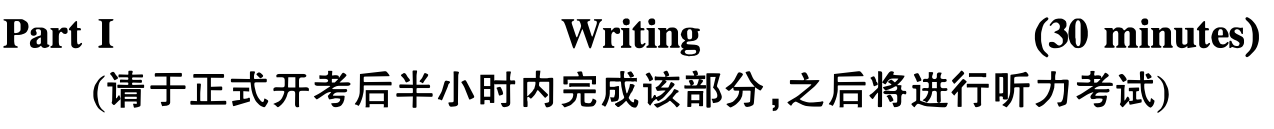
\includegraphics[width=\linewidth,height=.8\textheight,keepaspectratio]{2019-12-03.assets/char-009-line-000.png}\par

\textbf{Directions : }\textit{For this part , you are allowed 30 minutes to write an essay on the importance of}


\textit{having a sense of community responsibility. You should write at least 150 words but}


\textit{no more than 200 words.}


第 9／9页

\end{document}